\section{Systematic Uncertainties}\label{sec:ciSyst}

For each hypothesis test performed in this analysis, the null hypothesis is termed ``background-only'' and the alternative hypothesis is termed ``signal+background''.
Both of these hypotheses predict an event yield in a signal region.
The background-only hypothesis is derived from the background model described in Section \ref{sec:ciSig}.
The uncertainties corresponding to its prediction are the uncertainties on the background model, and are described in Section \ref{sec:ciSystBkg}.
Alternatively, the signal+background hypothesis also predicts a contribution to the event yield from a signal process.
The uncertainties corresponding to its prediction come both from the background model and the signal process; these are described in Sections \ref{sec:ciSystBkg} and \ref{sec:ciSystSig} respectively.
The groundwork for these uncertainties is described first in Section \ref{sec:ciSystVars}.

\subsection{Simulated Background Variations}\label{sec:ciSystVars}

A number of experimental and theoretical variations on the background shape are used in constructing the uncertainties on the background model and the signal processes.
The variations considered are due to theoretical and experimental uncertainties in the simulated background, as well as the uncertainties in the backgrounds from multi-jet and $W$+jets processes.
The largest source of uncertainty in the simulated background is theoretical, and it is particularly large at the high end of the dilepton mass spectrum.
The second largest source of uncertainty in the simulated background is experimental, and is mostly due to high-$p_\text{T}$ muon identification in the dimuon channel.
The third largest source is the uncertainty in the multi-jet and $W$+jets background components, and is estimated from the data.
Together, these uncertainties are referred to as \emph{systematic variations}, and are used to study the signal and background uncertainties.

\subsubsection{Theoretical Simulated Systematics}\label{sec:ciThySyst}

\begin{figure}[htp]
\centering
\subfloat[][]{{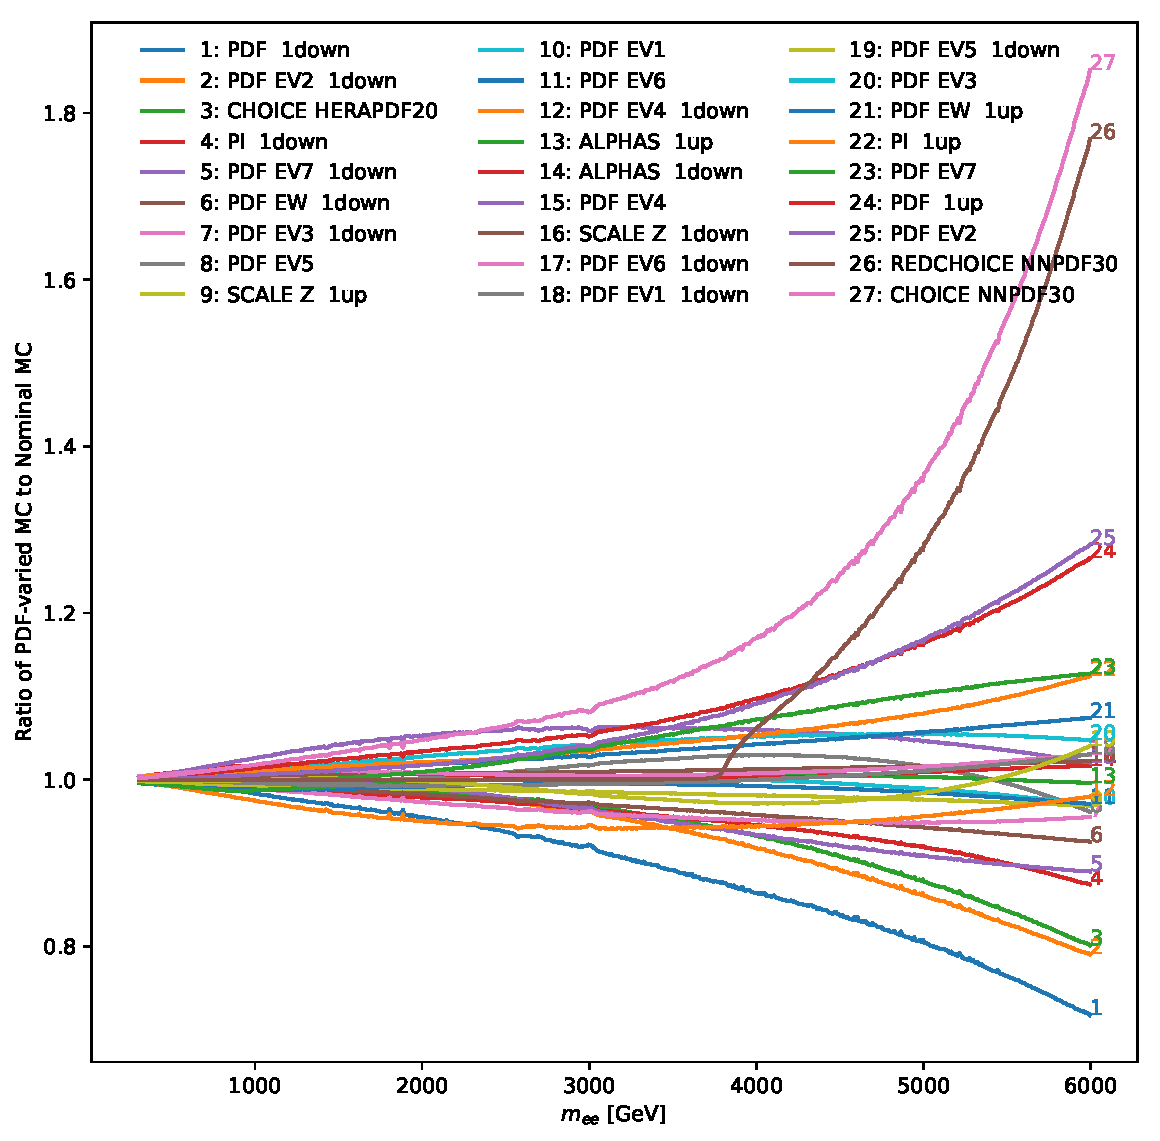
\includegraphics[width=0.45\textwidth]{figures/ci/bkgVarRatios/pdfComp-ee.pdf}}}
\subfloat[][]{{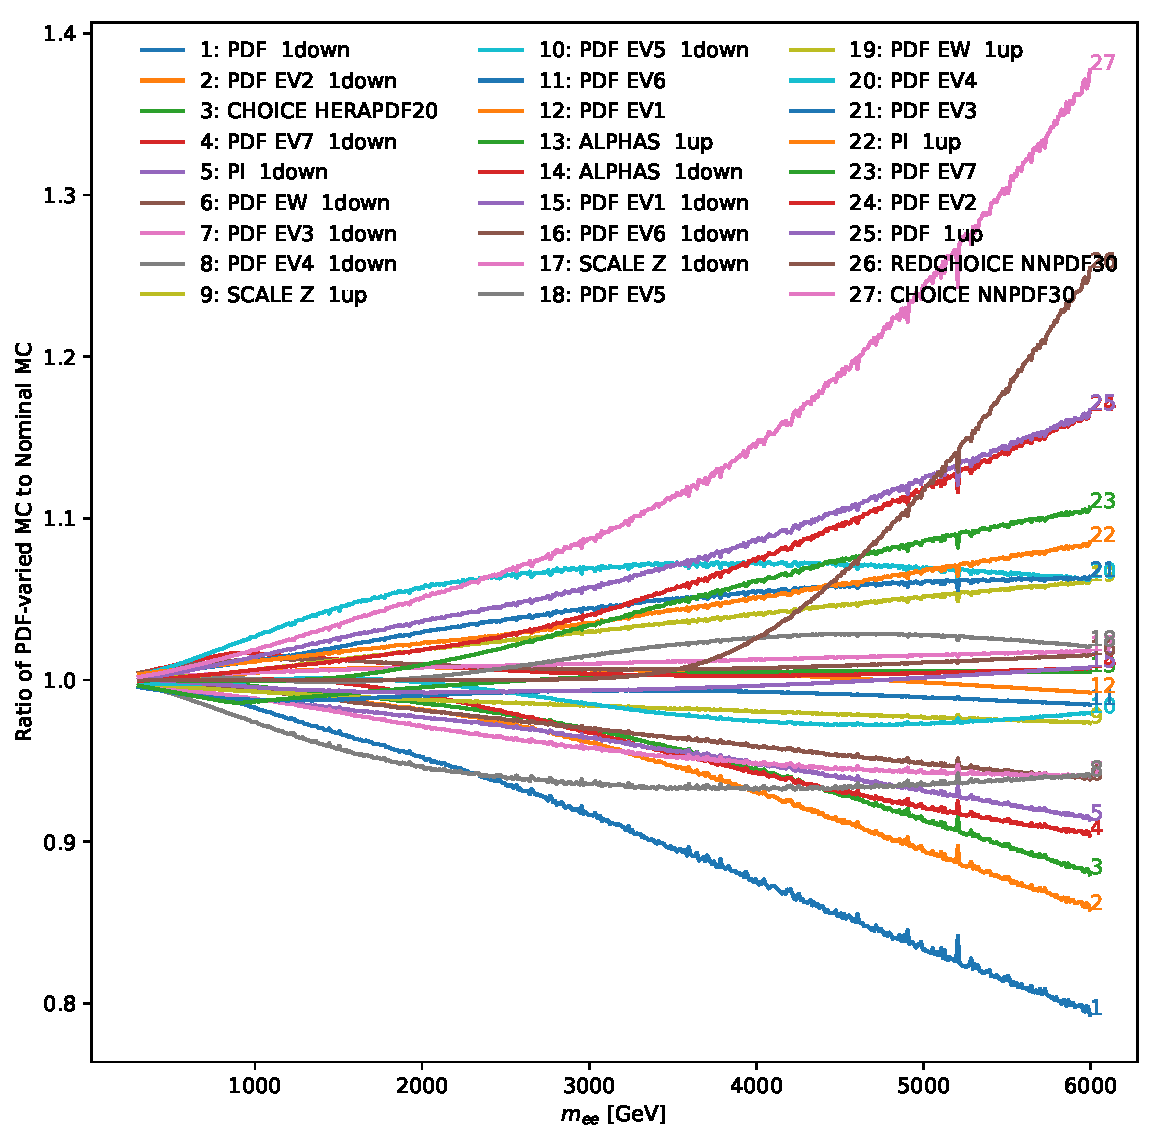
\includegraphics[width=0.45\textwidth]{figures/ci/bkgVarRatios/pdfComp-mm.pdf}}}
\caption{Illustration of theory variation shapes, shown as a ratio to the nominal MC, for $ee$ channel (a) and $\mu\mu$ channel (b). Two things are clear from these plots: the impact of the uncertainty in the PDF on $m_{ll}$, and that the impact grows with mass.}
\label{fig:ciThyVar}
\end{figure}

The following variations are considered for the theoretical uncertainties for the DY component only: the eigenvector variations of the nominal PDF set, variations of PDF scales, the strong coupling ($\alpha_{\textrm S}(M_Z)$), electroweak corrections, photon-induced corrections \cite{Martin:2005pi}, as well as the effect of choosing different PDF sets.
For all PDF variations, the modified DY component is used along with the other nominal background components.
These theoretical uncertainties are the same for both dilepton channels at generator level, but they result in different uncertainties at reconstruction level due to the different resolutions of the dielectron and dimuon channels.
% Further details of this procedure can be found in Ref.~\cite{EXOT-2016-05}.
The size of these uncertainties in the total simulated background is $\leq 19\%$ ($\leq 15\%$) below 4000~GeV for the dielectron (dimuon) channel.

The theoretical systematic uncertainties are used to produce variations on the invariant-mass spectra.
These are illustrated in Figure \ref{fig:ciThyVar}.


% \begin{table}[htp]
%     \centering
%     \begin{tabular}{c}
%     \toprule
%     PDF Variations \\
%     \midrule
%     ALPHAS \\
%     PDF EW \\
%     PI \\
%     PDF Eigenvector Variation 1 \\
%     PDF Eigenvector Variation 2 \\
%     PDF Eigenvector Variation 3 \\
%     PDF Eigenvector Variation 4 \\
%     PDF Eigenvector Variation 5 \\
%     PDF Eigenvector Variation 6 \\
%     PDF Eigenvector Variation 7 \\
%     SCALE Z \\
%     REDCHOICE NNPDF30 \\
%     CHOICE HERAPDF20  \\
%     CHOICE NNPDF30 \\
%     SCALE Z 1up \\
%     Without Run2 FakesTemplate \\
%     Run2 FakesTemplate x3 \\
%     Run2 FakesTemplate x2 \\
%     \bottomrule
%     \end{tabular}
%     \caption{Breakdown of variations of the nominal background included in the calculation of the ISS. These include the fake template variations, PDF choice, eigenvector and scale variations.}
%     \label{tab:ISSBreakdown}
% \end{table}

\subsubsection{Experimental Simulated Systematics}\ref{sec:ciExpSyst}

Uncertainty about the response and performance of the detector lead to systematic experimental uncertainties.
Among the experimental uncertainty sources in the dielectron channel, the dominant ones are the electron identification at low dielectron masses ($\leq 5\%$, below $\sim2000$~GeV) and the uncertainty in the electromagnetic energy scale at higher dielectron masses ($\leq 15\%$).
In the muon channel, the dominant experimental uncertainties arise from the muon reconstruction efficiency at low dimuon masses ($\leq 20\%$, below $\sim4000$~GeV) and from the identification of high-\pt muons at higher dimuon masses ($\leq 50\%$).
The full set of experimental uncertainties are illustrated for the electron channel in Figure \ref{fig:ciExpVarEe}, and for the muon channel in Figure \ref{fig:ciExpVarMm}.

\begin{figure}[htp]
\centering
\begin{overpic}[width=1\textwidth]{figures/ci/bkgVarRatios/pdfComp-ee-det.pdf}\put(85,0){}\end{overpic}
\caption{Ratio of the background variations to the nominal background estimate for the detector systematic variations in the electron channel. The prominent variations are numbered.}
\label{fig:ciExpVarEe}
\end{figure}

\begin{figure}[htp]
\centering
\begin{overpic}[width=1\textwidth]{figures/ci/bkgVarRatios/pdfComp-mm-det.pdf}\put(85,0){}\end{overpic}
\caption{Ratio of the background variations to the nominal background estimate for the detector systematic variations in the muon channel. The prominent variations are numbered.}
\label{fig:ciExpVarMm}
\end{figure}

\subsubsection{Multijet Electron Background}

The relative uncertainty of the simulated background due to the multi-jet and $W$+jets component rises from $\sim1\%$ at 1~TeV to $\sim10\%$ at 4~TeV.
For the multi-jet and $W$+jets component variations, the modified shape is used each time along with the other nominal background components from simulation.
This contribution is the smallest amongst all other variations in the CR.

\subsection{Background Estimate}\label{sec:ciSystBkg}
The background estimate describe in Section \ref{sec:ciBkg} predicts an event yield in the signal region, based on a functional form fit to the events observed in a control region.
Several assumptions are made in order to interpret this estimate as the prediction of the background hypothesis.
Each assumption is made with a degree of uncertainty.
This is quantified by the three systematic uncertainties described here: the extrapolation uncertainty, the induced spurious-signal (ISS) uncertainty, and the function bias uncertainty.

The extrapolation and ISS uncertainties are the dominant uncertainties on the background estimate.
These are both measured using statistical ensembles.

\subsubsection{Extrapolation Uncertainty}
\begin{figure}[h!]
\captionsetup[subfigure]{position=b}
\centering
\subfloat[][]{{\includegraphics[width=0.45\textwidth]{example-image-a}}}
\subfloat[][]{{\includegraphics[width=0.45\textwidth]{example-image-a}}} \\
\subfloat[][]{{\includegraphics[width=0.45\textwidth]{example-image-a}}}
\subfloat[][]{{\includegraphics[width=0.45\textwidth]{example-image-a}}}
\caption{Distributions of the differences between fits to the nominal dataset, and the toy datasets, for each SR.}
\label{fig:ciBkgEuSyst}
\end{figure}

The leading uncertainty on the estimated background is named the extrapolation uncertainty.
The functional form is fit in the CR to data collected in that region.
Since many events occupy each CR ($\approx$72k muons and $\approx$54k electrons), the shape of the \mll data distribution approximates the shape of the underlying truth-PDF that generated it.
However this approximation is not perfect due to statistical fluctuations in the CR.
The extrapolation uncertainty quantifies the degree to which statistical fluctuations in the CR may lead to varying background estimates in the SR.

This sort of uncertainty is present in other searches, and is sometimes called a ``function choice'' uncertainty.
Previously this has been estimated by comparing the result of choosing different functional forms to fit to the data.  {\color{red} [add citations, eg W']}
It is also possible to estimate this impact by looking at the constraints on and covariance of individual parameters of the functional form.
The procedure detailed here forgoes these estimates for a more direct measurement of the impact of statistical fluctuations on the estimated background.

To measure this impact, the background functional form is fit to the data in each CR.
This produces a smooth, \emph{nominal-PDF} that is the best available estimate of truth-PDF.
The background estimate from this fit in the SR defines $N_\text{bkg}^\text{Fit Nominal}$.
The nominal-PDF is used to generate an ensemble of \emph{pseudo-experiments}: toy datasets in the CR invariant-mass region with a multiplicity matching the dataset.
\footnote{There is no uncertainty as to the multiplicity of the actual dataset, and so this exactly determines the toy dataset multiplicity. An alternative option would be to allow $\sqrt{N}$ fluctuation of the multiplicity of each toys. In this case, the toy datasets correspond to the thought experiment: ``if Run 2 had been repeated, lasting for the same duration, what dataset may have been collected?'' This is not the precise thought experiment of interest. Instead, because a fixed number of events have already been sampled from the truth-PDF, it is asked: ``if an alternative sampling of the truth-PDF had taken place, what dataset may have been collected?''}
Each toy dataset is then fit using the background functional form and the resulting function is extrapolated to the SR to provide a toy background estimate $N_{\text{bkg},i}^\text{Fit Toy}$.
A comparison is made between the background estimate from the fit to the toy dataset and the nominal fit for each toy $i$:
\begin{equation*}
    \Delta_i^\text{stat}=N_{\text{bkg},i}^\text{Fit Toy}-N_\text{bkg}^\text{Fit Nominal}.
\end{equation*}
This defines the degree, $\Delta_i^\text{stat}$, to which statistical effects in the CR have altered the background estimate.


This procedure is repeated with an ensemble of 2000 toy datasets.
The distribution of $\Delta_i^\text{stat}$ values is built from each fit. These are shown in Figure \ref{eqn:ciBkgEuSyst} for each SR.
The standard deviation of these distributions is taken to define the systematic error on the background expectation due to the extrapolation uncertainty.

\subsubsection{Induced Spurious-Signal}
\begin{figure}[h!]
\captionsetup[subfigure]{position=b}
\centering
\subfloat[][]{{\includegraphics[width=0.45\textwidth]{example-image-a}}}
\subfloat[][]{{\includegraphics[width=0.45\textwidth]{example-image-a}}} \\
\subfloat[][]{{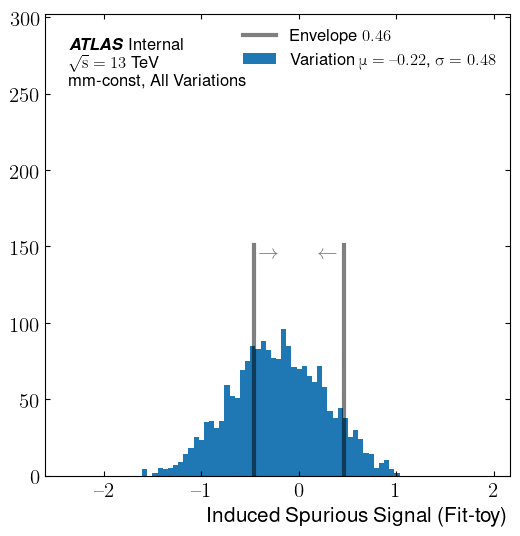
\includegraphics[width=0.45\textwidth]{figures/ci/iss/toyNSSDist-mm-const-all-noGaus.png}}}
\subfloat[][]{{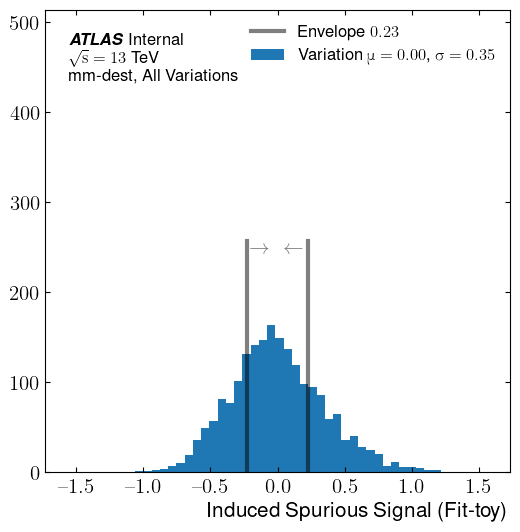
\includegraphics[width=0.45\textwidth]{figures/ci/iss/toyNSSDist-mm-dest-all-noGaus.png}}}
\caption{Distributions of the Induced Spurious-Signal.}
\label{fig:ciBkgIssSyst}
\end{figure}

% What needs to be measured
The sub-leading uncertainty on the background estimate is called the induced spurious-signal (ISS) uncertainty.
This quantifies the systematic difference between the background model and the true underlying background-only distribution in the SR.
The ISS how well the background model can be expected to model the underlying physical distribution from which the data has been sampled.
If the background functional form were to be fit to the true background-PDF, then the difference between the fitted function and normalized PDF in the CR is the ISS.
Since any missmodeling of the background, on average, leads to the identification of a signal even in the background-only scenario, this is missmodeling is called a \emph{spurious-signal}.

% Challenge with measuring it
The ISS can not be measured directly, since the background-PDF is unknown.
It is furthermore inaccurate to use the simulated background-only dataset to measure the ISS because this makes the improper assumption that the nominal simulation matches the shape of the true background-PDF.
Instead, a new methodology called the \emph{statistical background ensemble} was developed to measure the ISS.
The general theoretical motivation for the methodology is described in Appendix \ref{sec:backgroundEnsamble}.
The method seeks to measure the ISS from an ensemble of possible background shapes, each weighted by a prior likelihood.
The prior likelihoods are derived from the systematic variations discussed in Section \ref{sec:ciSystVars}.

The space of all plausible background shapes is described by linear combinations of the $n$ systematic variations.
Each of these is identified by a corresponding $n$-vector $\vec{\theta}$.
Each choice of $\vec{\theta}$ corresponds to a background shape $B'$:
\begin{equation}\begin{split}
    B'(\mll,\vec{\theta}) = B_\text{Nominal}(\mll) + \sum_{i=1}^n \omega_i(\mll)*\theta_i,
\end{split}\end{equation} 
where $\omega_i$ correspond to the shapes of the systematic variations.
The $\omega_i$ shapes can be normalized to correspond to $1\sigma$ deviations from the nominal shape.
In this case, $\theta_i=1$ corresponds to a $+1\sigma$ deviation, while $\theta_i=-1$ corresponds to a $-1\sigma$ deviation.
If the systematic variations are taken to define prior probabilities for nuisance parameters $\theta_i$, then the prior probability of $\vec{\theta}$ corresponding to the true background shape is:
\begin{equation}\begin{split}
    P(\vec{\theta})=\prod_{i=1}^n \text{G}(\theta_i),
\end{split}\end{equation} 
where $\text{G}(\theta_i)$ are standard normal functions.

In many cases, the systematic uncertainty shape is measured separately for upward and downward fluctuations.
For these systematics, the two shapes $\omega^+_i$ and $\omega^-_i$ are used as appropriate depending on whether $\theta_i$ is positive or negative.

Ideally, the ISS could be measured across the full space of $\vec{\theta}$.
This can be approximated numerically using an ensemble of backgrounds drawn from space of $\vec{\theta}$ randomly weighted by their prior likelihood.
For each of the $n$ systematic variations, a standard Gaussian PDF is sampled to determine the corresponding element of $\vec{\theta}$. \footnote{At the request of the ATLAS Publications Committee, the Gaussians are restricted to $[-1,1]$. This restriction is not impactful.}
The result is that each $\vec{\theta}$ of the ensemble is drawn with a probability proportional to the prior probability of the corresponding background shape.
Then, the background shapes $B'(\mll,\vec{\theta})$ and $B'(\mll,-\vec{\theta})$ are constructed.
The use of both $\vec{\theta}$ and $-\vec{\theta}$ forces a symmetric sampling of the space of $\vec{\theta}$. 
This reduces size of the ensemble required to sample the vector space.

This process is repeated to build an ensemble of background shapes, which are used to create 2000 Asimov toy datasets.
Each toy dataset is fit with the nominal background functional form.
A comparison is made between SR yields of the fitted function and the Asimov dataset for each toy $i$:
\begin{equation*}
    \Delta_i^\text{ISS}=N_{\text{bkg},i}^\text{Fit}-N_\text{bkg}^\text{Asimov}.
\end{equation*}
The distribution of $\Delta_i^\text{ISS}$ is built up through 2000 background shape toys for each SR, as shown in Figure \ref{fig:ciBkgIssSyst}.
The mean of these distributions defines the measurement of the ISS of the background model in each SR.
The width of these distributions is the uncertainty corresponding to that measurement.
The mean and standard deviation of the distribution are added in quadrature as the estimate of the ISS for the underlying background-PDF.

\subsubsection{Function Bias Uncertainty}

The final uncertainty on the background estimate is the function bias uncertainty.
This uncertainty constrains the degree to which a signal, if present in the CR, may bias the background expectation in the SR.
This is accomplished with the help of the S+B functional form of Equation \ref{eqn:ciSB}.
The results in Section \ref{sec:ciLinearity} establish that fits of the S+B functional form predict background yields in the SR that are not measurably distorted by the presence of a signal.
A comparison between the background expectations in the SR of the background-only and the S+B functional forms, when fitted to the data in the CR.
The difference between these two backgrounds expectations is taken to provide the function bias uncertainty.

The function bias uncertainty is small by construction.
If, when measured on data for a given control region, the value had been significant compared to extrapolation and ISS uncertainties, then this would have invalidated the choice of CR by indicating the presence of a signal-like feature.
In this case, a procedure was defined before unblinding the data in the SR.
The high-mass limit of the CR would be lowered until the bias vanished, with no adjustment to the SR. 
Because the non-resonant signals of interest vanish towards low-mass, reducing the upper limit of the CR would eventually remove the contribution from such a signal.

The results of the function bias measurement are shown in Figure \ref{fig:ciFuncBias}.
This measurement is repeated for each SR and for each chirality model.
A conservative choice of the largest bias for any given chirality is selected.
None of the function bias measurements are significant compared to the dominant uncertainties on the background model.
Indeed, the impact on the final results is under 2\%.

This uncertainty is only considered for the limits on the contact interaction energy scale \lam, since it depends on the shape of those signals.

\afterpage{
\begin{figure}[!htb]
\begin{center}
\subfloat[][]{{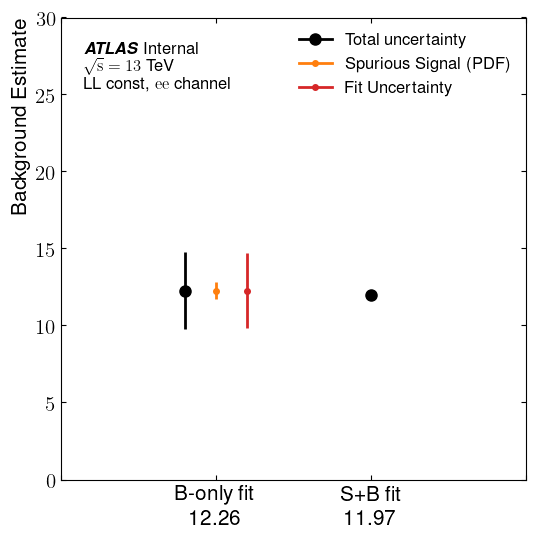
\includegraphics[width=0.24\textwidth]{figures/ci/bkgCompat-final/nbkg-LL-const-ee.png}}}
\subfloat[][]{{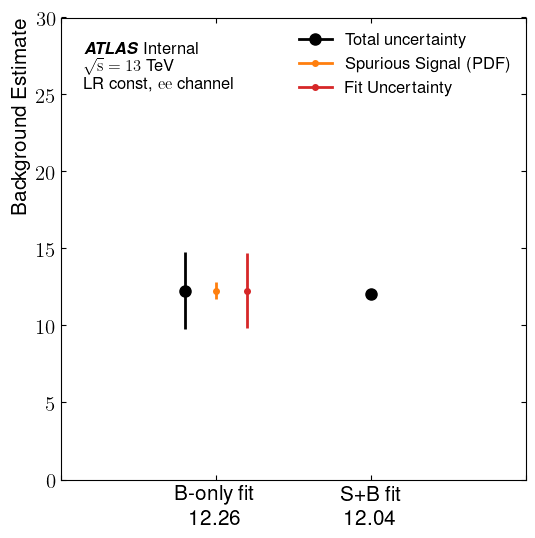
\includegraphics[width=0.24\textwidth]{figures/ci/bkgCompat-final/nbkg-LR-const-ee.png}}}
\subfloat[][]{{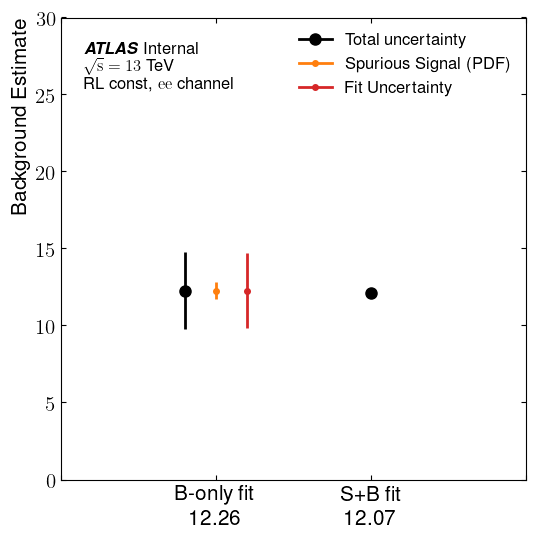
\includegraphics[width=0.24\textwidth]{figures/ci/bkgCompat-final/nbkg-RL-const-ee.png}}}
\subfloat[][]{{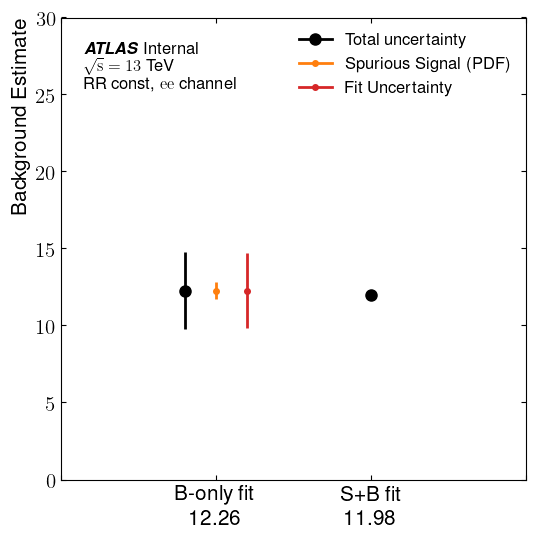
\includegraphics[width=0.24\textwidth]{figures/ci/bkgCompat-final/nbkg-RR-const-ee.png}}} \\
\subfloat[][]{{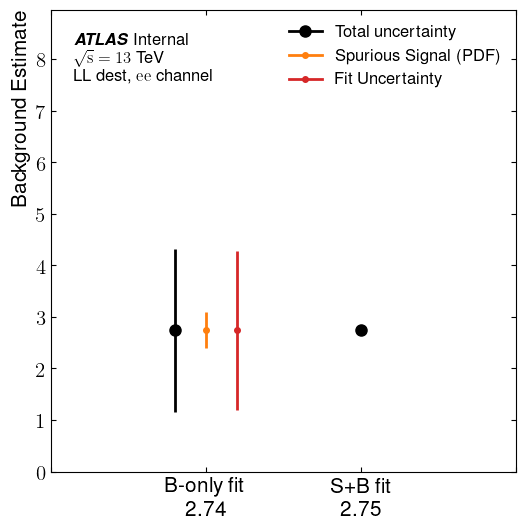
\includegraphics[width=0.24\textwidth]{figures/ci/bkgCompat-final/nbkg-LL-dest-ee.png}}}
\subfloat[][]{{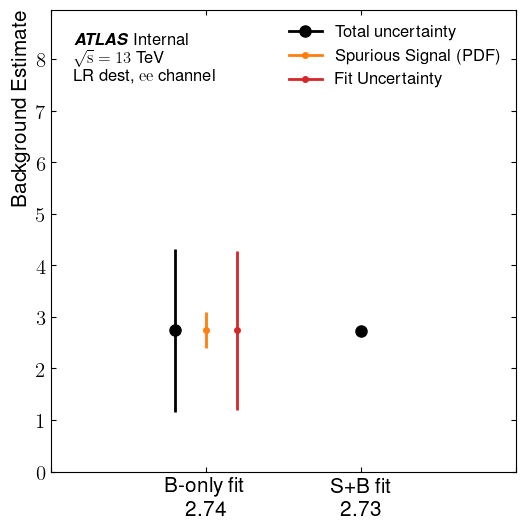
\includegraphics[width=0.24\textwidth]{figures/ci/bkgCompat-final/nbkg-LR-dest-ee.png}}}
\subfloat[][]{{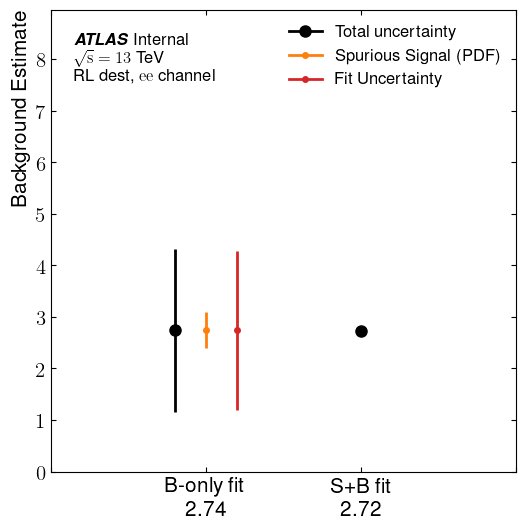
\includegraphics[width=0.24\textwidth]{figures/ci/bkgCompat-final/nbkg-RL-dest-ee.png}}}
\subfloat[][]{{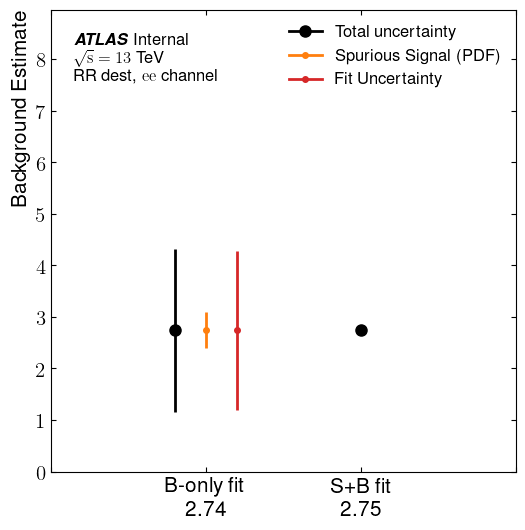
\includegraphics[width=0.24\textwidth]{figures/ci/bkgCompat-final/nbkg-RR-dest-ee.png}}} \\
\subfloat[][]{{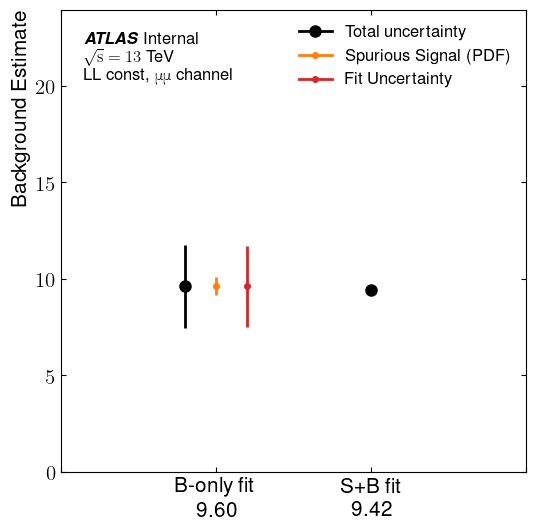
\includegraphics[width=0.24\textwidth]{figures/ci/bkgCompat-final/nbkg-LL-const-mm.png}}}
\subfloat[][]{{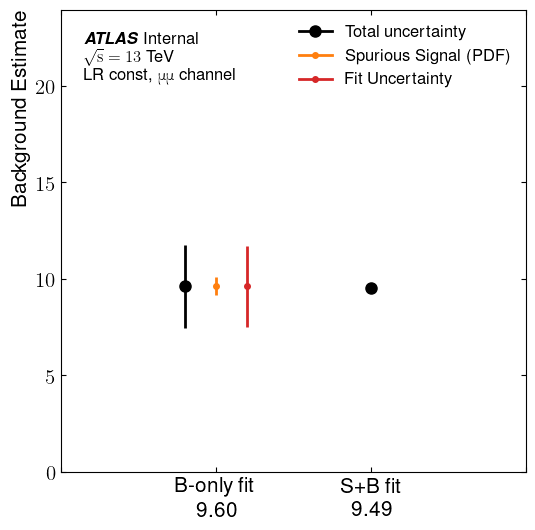
\includegraphics[width=0.24\textwidth]{figures/ci/bkgCompat-final/nbkg-LR-const-mm.png}}}
\subfloat[][]{{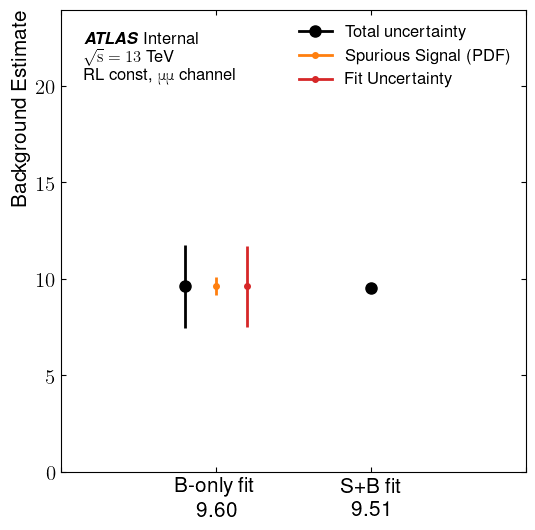
\includegraphics[width=0.24\textwidth]{figures/ci/bkgCompat-final/nbkg-RL-const-mm.png}}}
\subfloat[][]{{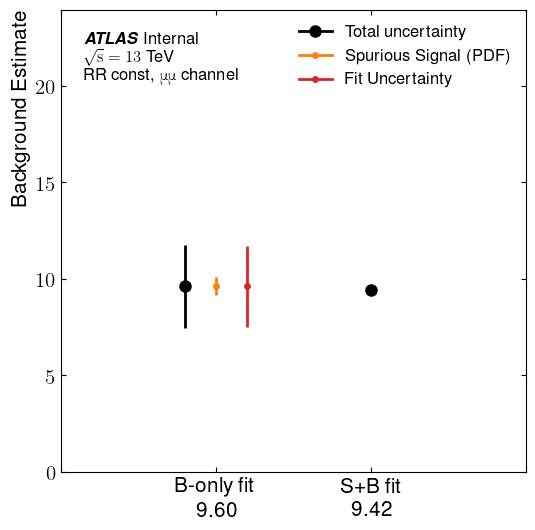
\includegraphics[width=0.24\textwidth]{figures/ci/bkgCompat-final/nbkg-RR-const-mm.png}}} \\
\subfloat[][]{{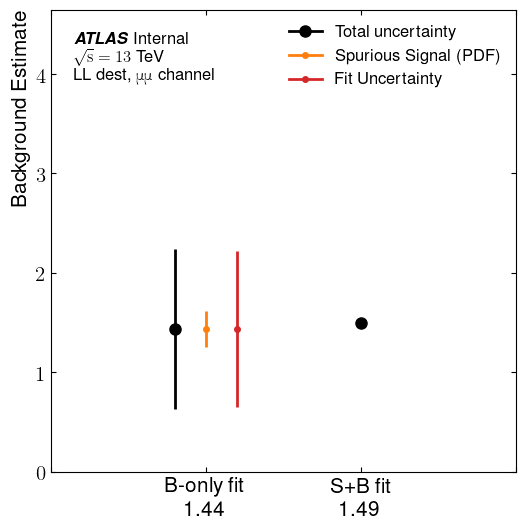
\includegraphics[width=0.24\textwidth]{figures/ci/bkgCompat-final/nbkg-LL-dest-mm.png}}}
\subfloat[][]{{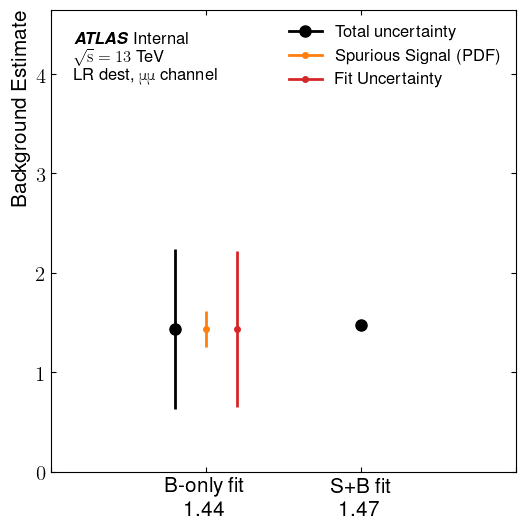
\includegraphics[width=0.24\textwidth]{figures/ci/bkgCompat-final/nbkg-LR-dest-mm.png}}}
\subfloat[][]{{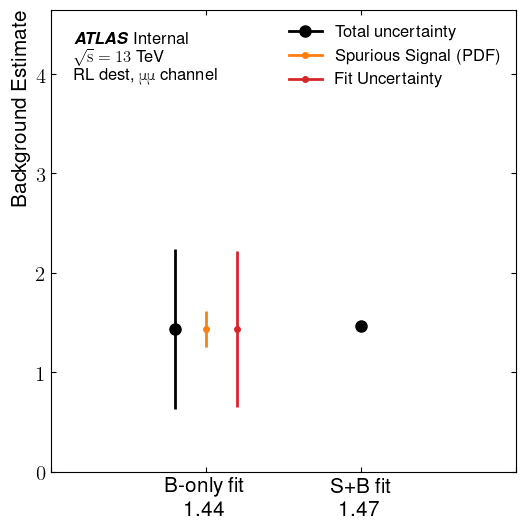
\includegraphics[width=0.24\textwidth]{figures/ci/bkgCompat-final/nbkg-RL-dest-mm.png}}}
\subfloat[][]{{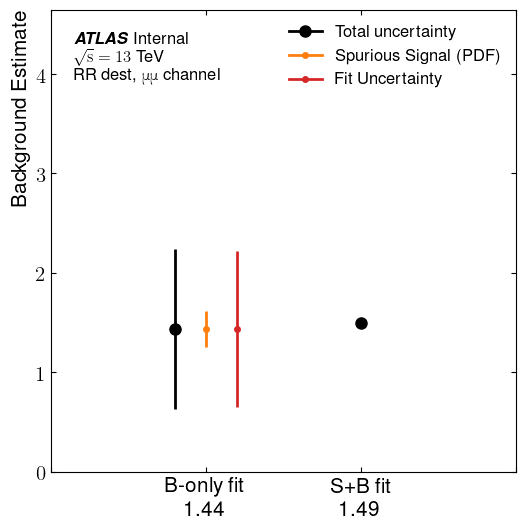
\includegraphics[width=0.24\textwidth]{figures/ci/bkgCompat-final/nbkg-RR-dest-mm.png}}}
\caption{Background estimate compared in the SR, for B-only and S+B fits to data in each channel. (a-d) show constructive \ee fits for LL, LR, RL, and RR chiralities. (d-h) show the same for destructive \ee. (i-l) show the same for constructive \mm, and (m-p) show the same for destructive \mm.}
\label{fig:ciFuncBias}
\end{center}
\end{figure}
\clearpage
}


\subsection{Signal Model}\label{sec:ciSystSig}
The signal models used in this analysis are more traditional than the background model, and therefore the corresponding systematic uncertainties are fairly standard.
There are both experimental and theoretical uncertainties to consider.
The experimental uncertainties, described in Section \ref{sec:ciSigExpSyst}, are applied similarly to the CI signal model, and the model-independent signal production.
The theoretical uncertainties, described in Section \ref{sec:ciSigThySyst}, must be considered differently.
The hypothesis test performed by this analysis compares the background hypothesis to the signal+background hypothesis.
The choice of the signal model unambiguous: there is no uncertainty in what signal model is being tested.
Theoretical variations, like the PDF choice and $\alpha_s$ scale are part of this signal model choice.
Different theoretical choices describe different signal models.
Therefore, these different signal models are tested for in separate hypothesis tests.

\subsubsection{Experimental}\label{sec:ciSigExpSyst}

The experimental uncertainties under consideration are described in Section \ref{sec:ciExpSyst}.
These are produced as functions of invariant-mass \mll.
The impact of each systematic on the CI signal model is the convolution of the CI shape in \mll and the systematic shape in \mll, but this is relatively independent of the signal shape.
For different contact interactions, the impact of experimental systematics generally varies by less than 1\%.
Thus for simplicity these are calculated for the LO DY shape in the CR and applied equally for each CI model.
The experimental uncertainties are given in Table \ref{tab:ciExpVariationBonanza}.
The sum in quadrature of the experimental uncertainties is used to constrain the signal prediction.
The experimental uncertainties of the signal are $\leq 9\%$ for the electron channel and $\leq 22\%$ for the muon channel.

\afterpage{
\begin{table}[]
\begin{center}
\caption{Impact of experimental uncertainties on NLO DY yield in CI signal regions. The sum in quadruature row includes only contributions from sources of impact $\geq 1\%$.}
\tiny
\begin{tabular}{|c|c|c|c|}
\hline
\hline
Process & Signal region & Uncertainty & \# events in SR \\
\hline
DY$\rightarrow ee$ & const. ($m_{ee} \geq 2200$ GeV) & nominal & $0.9824$ \\
DY$\rightarrow ee$ & const. ($m_{ee} \geq 2200$ GeV) & EG\_RES & $\sim 0.0\% \ \sim 0.0\%$ \\
DY$\rightarrow ee$ & const. ($m_{ee} \geq 2200$ GeV) & EG\_SCALE & $+ 5.9\% \   -5.8\%$ \\
DY$\rightarrow ee$ & const. ($m_{ee} \geq 2200$ GeV) & EL\_ChargeID & $\sim 0.0\% \ \sim 0.0\%$ \\
DY$\rightarrow ee$ & const. ($m_{ee} \geq 2200$ GeV) & EL\_ID & $+ 5.9\% \   -5.8\%$ \\
DY$\rightarrow ee$ & const. ($m_{ee} \geq 2200$ GeV) & EL\_Iso & $+ 0.8\% \   -0.8\%$ \\
DY$\rightarrow ee$ & const. ($m_{ee} \geq 2200$ GeV) & EL\_Reco & $+ 0.4\% \   -0.4\%$ \\
DY$\rightarrow ee$ & const. ($m_{ee} \geq 2200$ GeV) & EL\_TRIG\_EFF & $\sim 0.0\% \ \sim 0.0\%$ \\
DY$\rightarrow ee$ & const. ($m_{ee} \geq 2200$ GeV) & EL\_TRIG\_TOTAL & $\sim 0.0\% \ \sim 0.0\%$ \\
DY$\rightarrow ee$ & const. ($m_{ee} \geq 2200$ GeV) & PRW & $\sim 0.0\% \   -0.1\%$ \\
\hline
 & & Quad. sum (impact $\geq 1\%$) & $+ 8.4\% \   -8.2\%$ \\
\hline
DY$\rightarrow ee$ & dest. ($m_{ee} \geq 2770$ GeV) & nominal & $4.4867$ \\
DY$\rightarrow ee$ & dest. ($m_{ee} \geq 2770$ GeV) & EG\_RES & $\sim 0.0\% \ \sim 0.0\%$ \\
DY$\rightarrow ee$ & dest. ($m_{ee} \geq 2770$ GeV) & EG\_SCALE & $+ 5.2\% \   -4.9\%$ \\
DY$\rightarrow ee$ & dest. ($m_{ee} \geq 2770$ GeV) & EL\_ChargeID & $\sim 0.0\% \ \sim 0.0\%$ \\
DY$\rightarrow ee$ & dest. ($m_{ee} \geq 2770$ GeV) & EL\_ID & $+ 5.9\% \   -5.8\%$ \\
DY$\rightarrow ee$ & dest. ($m_{ee} \geq 2770$ GeV) & EL\_Iso & $+ 0.8\% \   -0.8\%$ \\
DY$\rightarrow ee$ & dest. ($m_{ee} \geq 2770$ GeV) & EL\_Reco & $+ 0.4\% \   -0.4\%$ \\
DY$\rightarrow ee$ & dest. ($m_{ee} \geq 2770$ GeV) & EL\_TRIG\_EFF & $\sim 0.0\% \ \sim 0.0\%$ \\
DY$\rightarrow ee$ & dest. ($m_{ee} \geq 2770$ GeV) & EL\_TRIG\_TOTAL & $\sim 0.0\% \ \sim 0.0\%$ \\
DY$\rightarrow ee$ & dest. ($m_{ee} \geq 2770$ GeV) & PRW & $\sim 0.0\% \ \sim 0.0\%$ \\
\hline
 & & Quad. sum (impact $\geq 1\%$) & $+ 7.9\% \   -7.6\%$ \\
\hline
\hline
DY$\rightarrow \mu\mu$ & const. ($m_{\mu\mu} \geq 2070$ GeV) & nominal & $1.3524$ \\
DY$\rightarrow \mu\mu$ & const. ($m_{\mu\mu} \geq 2070$ GeV) & MUON\_BADMUON\_STAT & $\sim 0.0\% \ \sim 0.0\%$ \\
DY$\rightarrow \mu\mu$ & const. ($m_{\mu\mu} \geq 2070$ GeV) & MUON\_BADMUON\_SYS & $+ 7.8\% \   -7.6\%$ \\
DY$\rightarrow \mu\mu$ & const. ($m_{\mu\mu} \geq 2070$ GeV) & MUON\_ISO\_STAT & $+ 0.3\% \   -0.3\%$ \\
DY$\rightarrow \mu\mu$ & const. ($m_{\mu\mu} \geq 2070$ GeV) & MUON\_ISO\_SYS & $+ 0.4\% \   -0.4\%$ \\
DY$\rightarrow \mu\mu$ & const. ($m_{\mu\mu} \geq 2070$ GeV) & MUON\_RECO\_STAT & $+ 0.6\% \   -0.6\%$ \\
DY$\rightarrow \mu\mu$ & const. ($m_{\mu\mu} \geq 2070$ GeV) & MUON\_RECO\_SYS & $+ 21.7\% \   -19.4\%$ \\
DY$\rightarrow \mu\mu$ & const. ($m_{\mu\mu} \geq 2070$ GeV) & MUON\_TTVA\_STAT & $\sim 0.0\% \ \sim 0.0\%$ \\
DY$\rightarrow \mu\mu$ & const. ($m_{\mu\mu} \geq 2070$ GeV) & MUON\_TTVA\_SYS & $\sim 0.0\% \ \sim 0.0\%$ \\
DY$\rightarrow \mu\mu$ & const. ($m_{\mu\mu} \geq 2070$ GeV) & MUON\_TRIG\_STAT & $\sim 0.0\% \ \sim 0.0\%$ \\
DY$\rightarrow \mu\mu$ & const. ($m_{\mu\mu} \geq 2070$ GeV) & MUON\_TRIG\_SYS & $+ 0.1\% \   -0.1\%$ \\
DY$\rightarrow \mu\mu$ & const. ($m_{\mu\mu} \geq 2070$ GeV) & MUON\_ID & $+ 1.0\% \   -1.1\%$ \\
DY$\rightarrow \mu\mu$ & const. ($m_{\mu\mu} \geq 2070$ GeV) & MUON\_MS & $+ 4.6\% \   -3.7\%$ \\
DY$\rightarrow \mu\mu$ & const. ($m_{\mu\mu} \geq 2070$ GeV) & MUON\_SAGITTA\_RESBIAS & $+ 12.8\% \ + 5.5\%$ \\
DY$\rightarrow \mu\mu$ & const. ($m_{\mu\mu} \geq 2070$ GeV) & MUON\_SAGITTA\_RHO & $\sim 0.0\% \ \sim 0.0\%$ \\
DY$\rightarrow \mu\mu$ & const. ($m_{\mu\mu} \geq 2070$ GeV) & MUON\_SCALE & $  -0.4\% \ + 0.3\%$ \\
DY$\rightarrow \mu\mu$ & const. ($m_{\mu\mu} \geq 2070$ GeV) & PRW & $\sim 0.0\% \ \sim 0.0\%$ \\
\hline
 & & Quad. sum (impact $\geq 1\%$) & $+ 26.7\% \   -21.9\%$ \\
\hline
DY$\rightarrow \mu\mu$ & dest. ($m_{\mu\mu} \geq 2570$ GeV) & nominal & $4.7216$ \\
DY$\rightarrow \mu\mu$ & dest. ($m_{\mu\mu} \geq 2570$ GeV) & MUON\_BADMUON\_STAT & $\sim 0.0\% \ \sim 0.0\%$ \\
DY$\rightarrow \mu\mu$ & dest. ($m_{\mu\mu} \geq 2570$ GeV) & MUON\_BADMUON\_SYS & $+ 4.0\% \   -3.8\%$ \\
DY$\rightarrow \mu\mu$ & dest. ($m_{\mu\mu} \geq 2570$ GeV) & MUON\_ISO\_STAT & $+ 0.3\% \   -0.2\%$ \\
DY$\rightarrow \mu\mu$ & dest. ($m_{\mu\mu} \geq 2570$ GeV) & MUON\_ISO\_SYS & $+ 0.5\% \   -0.3\%$ \\
DY$\rightarrow \mu\mu$ & dest. ($m_{\mu\mu} \geq 2570$ GeV) & MUON\_RECO\_STAT & $+ 0.6\% \   -0.5\%$ \\
DY$\rightarrow \mu\mu$ & dest. ($m_{\mu\mu} \geq 2570$ GeV) & MUON\_RECO\_SYS & $+ 17.9\% \   -16.1\%$ \\
DY$\rightarrow \mu\mu$ & dest. ($m_{\mu\mu} \geq 2570$ GeV) & MUON\_TTVA\_STAT & $+ 0.1\% \ \sim 0.0\%$ \\
DY$\rightarrow \mu\mu$ & dest. ($m_{\mu\mu} \geq 2570$ GeV) & MUON\_TTVA\_SYS & $\sim 0.0\% \ \sim 0.0\%$ \\
DY$\rightarrow \mu\mu$ & dest. ($m_{\mu\mu} \geq 2570$ GeV) & MUON\_TRIG\_STAT & $+ 0.2\% \ \sim 0.0\%$ \\
DY$\rightarrow \mu\mu$ & dest. ($m_{\mu\mu} \geq 2570$ GeV) & MUON\_TRIG\_SYS & $+ 0.2\% \ \sim 0.0\%$ \\
DY$\rightarrow \mu\mu$ & dest. ($m_{\mu\mu} \geq 2570$ GeV) & MUON\_ID & $+ 0.7\% \   -0.7\%$ \\
DY$\rightarrow \mu\mu$ & dest. ($m_{\mu\mu} \geq 2570$ GeV) & MUON\_MS & $+ 2.7\% \   -2.2\%$ \\
DY$\rightarrow \mu\mu$ & dest. ($m_{\mu\mu} \geq 2570$ GeV) & MUON\_SAGITTA\_RESBIAS & $+ 8.0\% \ + 1.8\%$ \\
DY$\rightarrow \mu\mu$ & dest. ($m_{\mu\mu} \geq 2570$ GeV) & MUON\_SAGITTA\_RHO & $\sim 0.0\% \ \sim 0.0\%$ \\
DY$\rightarrow \mu\mu$ & dest. ($m_{\mu\mu} \geq 2570$ GeV) & MUON\_SCALE & $  -0.4\% \ + 0.4\%$ \\
DY$\rightarrow \mu\mu$ & dest. ($m_{\mu\mu} \geq 2570$ GeV) & PRW & $\sim 0.0\% \ + 0.2\%$ \\
\hline
\hline
\end{tabular}
\label{tab:ciExpVariationBonanza}
\end{center}
\end{table}
\clearpage
}

\subsubsection{Theoretical}\label{sec:ciSigThySyst}
The theoretical uncertainties under consideration are described in Section \ref{sec:ciThySyst}.
These are useful in order to provide alternative signal models that correspond to the $1\sigma$ limits on theoretical parameters.
The impact of the theoretical uncertainties on the signal yield is calculated in each SR.
It is equal to the sum in quadrature of the convolution of the theory systematic shapes with the LO DY shape.


\subsection{Summary}

The numerical values of the uncertainties are given in Table \ref{tab:ciUncerts}.
For all cases, the relative uncertainties in the destructive SRs are larger than those in the constructive SRs.
This is due to both the smaller size of the SR leading to less background and hence larger relative uncertainty, and the smaller size of the CR leading to a weaker constraint on the background model.
For the background estimates, the leading uncertainty in each SR is the extrapolation uncertainty, followed by the ISS uncertainty.
Many of the experimental and theoretical systematics are measured separately for upward and downward fluctuations.


\begin{table}[!h]
\begin{center}
\caption{Summary of the relative uncertainties in the background estimate and signal in each SR, where EU is the `extrapolation uncertainty', ISS is the `induced spurious-signal uncertainty' and FB is the `function bias uncertainty'. Experimental and theoretical uncertainties are shown as well, with the latter averaged across CI chirality scenarios and quoted for $\Lambda=30$~TeV only.}
\begingroup
\setlength{\tabcolsep}{10pt} % Default value: 6pt
\renewcommand{\arraystretch}{1.5} % Default value: 1
{\small
% \begin{tabular}{l l | r r r | r r r r}
\begin{tabular}{l l | r r r | r@{}l r@{}l}
% \Xhline{2\arrayrulewidth}
\toprule
\multirow{2}{*}{Channel} & \multirow{2}{*}{Interference} & \multicolumn{3}{c|}{Background uncertainties} & \multicolumn{4}{c}{Signal uncertainties}\\
        &              & $\sigma_b^\text{EU}$ & $\sigma_b^\text{ISS}$ & $\sigma_b^\text{FB}$ & \multicolumn{2}{c}{$\sigma_s^\text{Experiment}$} & \multicolumn{2}{c}{$\sigma_s^\text{Theory}$} \\
\midrule
\ee     & Constructive & 14\% & 4\%  & 2\% & 8&\%                               & \makecell[r]{+11 \\ --10}&\makecell[l]{\% \\ \%} \\
\ee     & Destructive  & 34\% & 7\% & 1\%  & 8&\%                               & \makecell[r]{+14 \\ --13}&\makecell[l]{\% \\ \%} \\
$\mm$ & Constructive & 21\% & 6\%  & 2\% & \makecell[r]{+20 \\ --17}&\makecell[l]{\% \\ \%} & \makecell[r]{+10 \\ --9}&\makecell[l]{\% \\ \%} \\
$\mm$ & Destructive  & 58\% & 24\% & 4\% & \makecell[r]{+27 \\ --22}&\makecell[l]{\% \\ \%} & \makecell[r]{+13 \\ --12}&\makecell[l]{\% \\ \%} \\
% \Xhline{2\arrayrulewidth}
\bottomrule
\end{tabular}
}
\endgroup
\label{tab:ciUncerts}
\end{center}
\end{table}
